% !TEX root = ../../../main.tex
% 所属：第一部分：单变量分析学 / 第7章：微分法
% 节：7.7 L'Hospital法则
% 正文按原文件顺序保存；由 ../chapter7.tex 调用。
\section{L'Hospital法则}
\begin{center}
	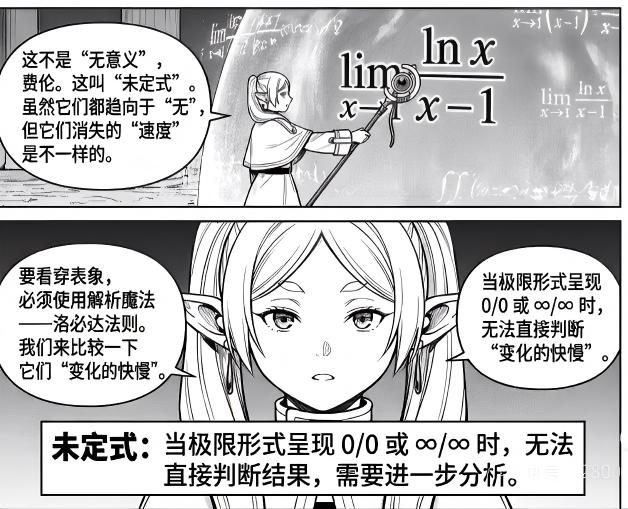
\includegraphics[width=0.7\linewidth]{figure/C6/222}
\end{center}
L'Hospital 法则用于处理函数极限的待定型$(\dfrac{\star}{\infty},\dfrac{0}{0})$
\begin{definition}
	(L'Hospital 法则)设 $f(x), g(x) \in D(a,a+d]$， $g'(x) \neq 0$.且下列条件之一成立：
	
	1.$\lim\limits_{x \to a^+} f(x) = \lim\limits_{x \to a^+} g(x) = 0$
	
	2.$	\lim\limits_{x \to a^+} g(x) = \pm \infty \text{ 或 } \infty$
	
	则有
	\[
	\lim_{x \to a^+} \frac{f(x)}{g(x)} = \lim_{x \to a^+} \frac{f'(x)}{g'(x)}
	\]
	
	
\end{definition}
注：此结论对以下极限行为均有效：
\[
x \to a^+, x \to a^-, x \to a, x \to \infty, x \to -\infty, x \to +\infty
\]

在相应的邻域内，有各自的洛必达法则成立.这里以 $x \to a^+$ 为例.
\begin{proof}
	先考虑 $\lim\limits_{x \to a^+} \dfrac{f'(x)}{g'(x)}$ 存在且有限的情况.设$\lim\limits_{x \to a^+} \dfrac{f'(x)}{g'(x)}=A$
	
	若满足情况1，令
	\[
	\ \widetilde{f}(x) = \begin{cases}
		0 & x = a, \\
		f(x) & x \in (a, a+d],
	\end{cases}
	\quad
	\widetilde{g}(x) = \begin{cases}
		0 & x = a, \\
		g(x) & x \in (a, a+d].
	\end{cases}
	\]
	
	$\widetilde{f}, \widetilde{g}\in C(a, a+d]$, 且对于 $x \in (a, a+d]$, $\widetilde{f}'(x) = f'(x)$, $\widetilde{g}'(x) = g'(x)$.
	
	由 $g'(x) \neq 0$ 及 Rolle 定理，$g(x)$ 在 $(a, a+d]$ 上至多有一个零点.
	必要时缩小 $d$，可设 $g(x) \neq 0$ 对一切 $x \in (a, a+d]$ 成立，从而 Cauchy 中值定理的条件满足.
	
	由 $\widetilde{f}(a) = \widetilde{g}(a) = 0$，对于 $x \in (a, a+d]$，
	\[
	\frac{f(x)}{g(x)} = \frac{\widetilde{f}(x) - \widetilde{f}(a)}{\widetilde{g}(x) - \widetilde{g}(a)}
	\]
	
	由 Cauchy 中值定理，$\exists \xi \in (a, x)$, 使得
	\[
	\frac{f(x)}{g(x)} = \frac{\widetilde{f}(x) - \widetilde{f}(a)}{\widetilde{g}(x) - \widetilde{g}(a)} = \frac{\widetilde{f}'(\xi)}{\widetilde{g}'(\xi)} = \frac{f'(\xi)}{g'(\xi)}
	\]
	
	当 $x \to a^+$ 时，$\xi \to a^+$，故
	\[
	\lim_{x \to a^+} \frac{f(x)}{g(x)} = \lim_{x \to a^+} \frac{f'(\xi)}{g'(\xi)}
	\]
	
	情况 2
	
	取 $x_0 \in(a, a+d]$ 且 $x_0$ 充分靠近 $a$ ．
	$$
	\begin{aligned}
		&\frac{f(x)}{g(x)}=\frac{f(x)-f\left(x_0\right)}{g(x)}+\frac{f\left(x_0\right)}{g(x)}=\frac{f(x)-f\left(x_0\right)}{g(x)-g\left(x_0\right)} \cdot \frac{g(x)-g\left(x_0\right)}{g(x)}+\frac{f\left(x_0\right)}{g(x)} \\
		&\frac{f(x)}{g(x)}-A=\left[\frac{f(x)-f\left(x_0\right)}{g(x)-g\left(x_0\right)}-A\right]\left(1-\frac{g\left(x_0\right)}{g(x)}\right)+A\left(1-\frac{g\left(x_0\right)}{g(x)}\right)+\frac{f\left(x_0\right)}{g(x)}-A \\
		&\left|\frac{f(x)}{g(x)}-A\right| \leqslant\left|\frac{f(x)-f\left(x_0\right)}{g(x)-g\left(x_0\right)}-A\right|\left|1-\frac{g\left(x_0\right)}{g(x)}\right|+\left|\frac{f\left(x_0\right)-A g\left(x_0\right)}{g(x)}\right|\quad(*)
	\end{aligned}
	$$
	
	$\exists \xi $介于$x, x_0$ 之间，使得
	\[
	\frac{f(x) - f(x_0)}{g(x) - g(x_0)} = \frac{f'(\xi)}{g'(\xi)}
	\]
	
	当 $x_0 \to a^+,x \to a^+$, $\xi \to a^+$, 由 $\lim\limits_{x \to a^+} \dfrac{f'(x)}{g'(x)} = A$，$\forall \varepsilon > 0$, $\exists \delta > 0$，当 $x \in (a, a+\delta)$ 时，
	\[
	\left|\frac{f'(x)}{g'(x)} - A\right| < \varepsilon
	\]
	
	取 $x \in (a, a+\delta)$，则 $\xi \in (a, a+\delta) \subset (a, a+d)$，
	\[
	\left|\frac{f'(\xi)}{g'(\xi)} - A\right| < \eps
	\]
	
	代入 $(*)$，
	\[
	\left|\frac{f(x)}{g(x)} - A\right| \leqslant 
	\eps \left|1 - \frac{g(x_0)}{g(x)}\right|+\left|\frac{f(x_0) - A g(x_0)}{g(x)}\right|
	\]
	
	对上述 $x_0$，
	\[
	\lim_{x \to a^+} \left(1 - \frac{g(x_0)}{g(x)}\right) = 1, \quad \lim_{x \to a^+} \frac{f(x_0) - A g(x_0)}{g(x)} = 0
	\]
	
	$\exists \rho$ 使得 $0 < \rho < \delta$，使得 $x \in (a, a+\rho)$ 时，
	\[
	\left|1 - \frac{g(x_0)}{g(x)}\right| < 1 + \frac{\eps}{2}, \quad \left|\frac{f(x_0) - A g(x_0)}{g(x)}\right| < \frac{\eps}{2}
	\]
	
	则
	\[
	\left|\frac{f(x)}{g(x)} - A\right| < \eps \left(1 + \frac{\eps}{2}\right) + \frac{\eps}{2}
	\]
	
	故
	\[
	\lim_{x \to a^+} \frac{f(x)}{g(x)} = A
	\]
	
	下面考虑 $\lim\limits_{x \to a^+} \dfrac{f'(x)}{g'(x)} = \pm\infty$ 的情况.从 $+\infty$ 为例.
	
	情况1: $\lim\limits_{x \to a^+} f(x) = \lim\limits_{x \to a^+} g(x) = 0$，考虑 $(a, a+d]$.
	
	令
	\[
	\ \widetilde{f}(x) = \begin{cases}
		0 & x = a, \\
		f(x) & x \in (a, a+d],
	\end{cases}
	\quad
	\widetilde{g}(x) = \begin{cases}
		0 & x = a, \\
		g(x) & x \in (a, a+d].
	\end{cases}
	\]
	
	由 $\lim\limits_{x \to a^+} \dfrac{f'(x)}{g'(x)} = +\infty$，$\forall G > 0$, $\exists \delta > 0$，$\forall x \in (a, a+\delta)$，使
	\[
	\frac{f'(x)}{g'(x)} > G
	\]
	
	由 Cauchy 中值定理，$\exists \xi \in (a, a+\delta)$ 使
	\[
	\frac{f(x)}{g(x)} = \frac{\widetilde{f}(x) - \widetilde{f}(a)}{\widetilde{g}(x) - \widetilde{g}(a)} = \frac{f'(\xi)}{g'(\xi)} > G
	\]
	
	故
	\[
	\lim_{x \to a^+} \frac{f(x)}{g(x)} = +\infty
	\]
	
	情况2: 设 $\lim\limits_{x \to a^+} g(x) = \infty$.任取 $x_0 \in (a, a+\delta)$, $\delta_1 \in (0, x_0 - a)$.使得当 $x \in (a, a+\delta_1)$ 时
	
	\[
	\max \left\{ \left|\dfrac{g(x_0)}{g(x)}\right|, \left|\dfrac{f(x_0)}{g(x)}\right|\right\} \leqslant \frac{1}{2}
	\]
	
	由
	\[
	\frac{f(x)}{g(x)} = \left[1 - \frac{g(x_0)}{g(x)}\right] \frac{f(x) - f(x_0)}{g(x) - g(x_0)} + \frac{f(x_0)}{g(x)}	= \left[1 - \frac{g(x_0)}{g(x)}\right] \frac{f'(\xi)}{g'(\xi)} + \frac{f(x_0)}{g(x)}
	\]
	对 $x \in (a, a+\delta_1)$ 时
	\[
	\left|\frac{f(x)}{g(x)}\right| \geqslant \frac{1}{2}(G + 1) - \frac{1}{2} = \frac{G}{2}
	\]
	
	故
	\[
	\lim_{x \to a^+} \frac{f(x)}{g(x)} = +\infty
	\]
	
\end{proof}

